\documentclass[11pt,a4paper]{article}

\usepackage{amsmath,amssymb,amsthm}
\usepackage{mathtools}
\usepackage{geometry}
\usepackage{hyperref}
\usepackage{xcolor}
\usepackage{tikz}
\usetikzlibrary{arrows.meta,positioning,decorations.markings,calc}
\usepackage{tcolorbox}
\tcbuselibrary{skins,breakable}
\usepackage{enumitem}
\usepackage{microtype}

\geometry{margin=2.3cm}
\hypersetup{colorlinks=true,linkcolor=blue!60!black,urlcolor=blue!60!black}

\definecolor{commentboxbg}{RGB}{240,245,250}
\newtcolorbox{commentbox}[1][]{
  colback=commentboxbg, colframe=blue!50!black,
  fonttitle=\bfseries, title=Commentary, breakable, #1
}

% Excitation rail in blue, bare rail in black; bridge dashed.
\newcommand{\Gex}{(-i\omega+V_{0}+r)^{-1}}
\newcommand{\Gba}{(-i\omega+r)^{-1}}

\title{\vspace{-1.2cm}Cleaner diagrammatic rules --- reply\\[2pt]
{\large On Gunnar's note of 9~May 2026}}
\author{Sirsh \& Claude}
\date{9 May 2026}

\begin{document}
\maketitle

\vspace{-1em}
\begin{commentbox}[title=One-line takeaway]
You're right that my 7~May note had a misunderstanding: I dropped the $V_{0}$
shift on the excitation rail, and I claimed flip vertices don't generate
loops. Both errors live in the \emph{kernel} half of the note (\S 3). The
\emph{combinatorial} half (Laplacian, generating function, marking, Schur,
asymptotics) is untouched by the error and survives verbatim. Below: your
rules and atlas, faithfully reproduced; the precise location of the
misunderstanding; what survives; and a small worry about
``odd-$m$ diagrams cancel pairwise.''
\end{commentbox}

%==================================================
\section{Your rules, as I now read them}
%==================================================

An $n$-rail diagram with rails $i\in\{0,1,\dots,n{-}1\}$. Rail $i{=}0$
is the special ``excitation rail''; the excitation enters on the right
and leaves on the left. Every rail is a continuous line passing through
every vertex.

\begin{itemize}[leftmargin=2em,itemsep=2pt]
\item \textbf{Propagator on a rail segment depends on whether it carries
the excitation:}
\[
\text{with excitation:}\;\;\Gex,\qquad
\text{without:}\;\;\Gba.
\]
Only rail $0$ has external $\omega$ entering and leaving; all other rails
have no net $\omega$-flux.

\item \textbf{Vertex is a 4-leg object:} two rails $i,j$ pass through; a
dashed bridge connects them. Two flavours, both symmetric in $i\leftrightarrow j$:
\begin{itemize}[leftmargin=1.4em,itemsep=1pt]
\item \emph{stay vertex} ($+v_{ij}$): the excitation continues on the rail
it was on.
\item \emph{flip vertex} ($-v_{ij}$): the excitation hops to the other rail.
\end{itemize}
Both vertices carry $\omega$; loops are integrated over.
\end{itemize}

In every diagram below, the rail segment carrying the excitation is
\textcolor{blue!70!black}{\textbf{thick blue}}; bare segments are thin
black; bridges are dashed. The excitation worldline is therefore the
unique connected blue path from right to left.

%==================================================
\section{Your atlas, faithfully reproduced}\label{sec:atlas}
%==================================================

I run through your six diagrams with the rule that, on every \emph{segment}
between consecutive vertices, the propagator is $\Gex$ if the segment is
blue and $\Gba$ otherwise.

\paragraph{$n{=}2,\;m{=}0$.}
\begin{center}
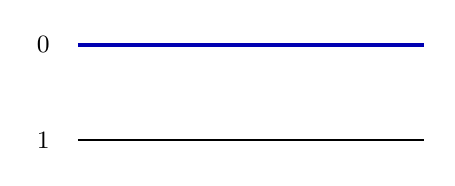
\begin{tikzpicture}[scale=1.1]
  \draw[ultra thick,blue!70!black] (-2,0.55)--(2,0.55);
  \draw[thick] (-2,-0.55)--(2,-0.55);
  \node at (-2.4,0.55){\small$0$}; \node at (-2.4,-0.55){\small$1$};
\end{tikzpicture}
\end{center}
\[
\Gamma \;\widehat=\; \Gex.
\]

\paragraph{$n{=}2,\;m{=}1$ (stay, bridge to rail $1$).}
\begin{center}
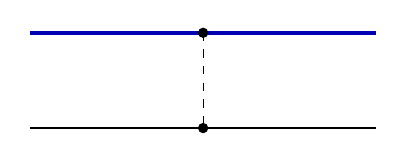
\begin{tikzpicture}[scale=1.1]
  \draw[ultra thick,blue!70!black] (-2,0.55)--(2,0.55);
  \draw[thick] (-2,-0.55)--(2,-0.55);
  \draw[dashed] (0,0.55)--(0,-0.55);
  \filldraw (0,0.55) circle (1.5pt);
  \filldraw (0,-0.55) circle (1.5pt);
\end{tikzpicture}
\end{center}
\[
\Gamma \;\widehat=\; \Gex\; v_{01}\;\Gex.
\]
(Rail $1$ has zero net $\omega$-flux: its outer segments contribute
$1/r$ each, normalisation absorbed.)

\paragraph{$n{=}2,\;m{=}2$, two stays.}
The excitation stays on rail~$0$; two bridges visit rail $1$. The two
bridges close a single loop whose top leg is rail-$0$-with-excitation and
bottom leg is rail-$1$-bare:
\begin{center}
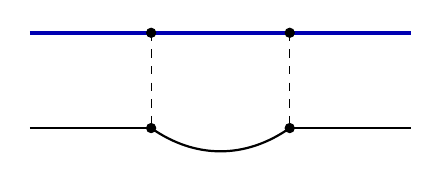
\begin{tikzpicture}[scale=1.1]
  \draw[ultra thick,blue!70!black] (-2.2,0.55)--(2.2,0.55);
  \draw[thick] (-2.2,-0.55)--(-0.8,-0.55);
  \draw[thick] (0.8,-0.55)--(2.2,-0.55);
  \draw[thick] (-0.8,-0.55) to[bend right=35] (0.8,-0.55);
  \draw[dashed] (-0.8,0.55)--(-0.8,-0.55);
  \draw[dashed] ( 0.8,0.55)--( 0.8,-0.55);
  \filldraw (-0.8,0.55) circle (1.5pt);
  \filldraw ( 0.8,0.55) circle (1.5pt);
  \filldraw (-0.8,-0.55) circle (1.5pt);
  \filldraw ( 0.8,-0.55) circle (1.5pt);
\end{tikzpicture}
\end{center}
\begin{align*}
\Gamma \;&\widehat=\; \Gex\,v_{01}^{2}\,\Gex
\;\times\;\int\!\frac{d\omega'}{2\pi}\,
\big(-i(\omega+\omega')+V_{0}+r\big)^{-1}\big(i\omega'+r\big)^{-1}\\
&=\;\Gex\,v_{01}^{2}\,\Gex\,(-i\omega+V_{0}+2r)^{-1}.
\end{align*}

\paragraph{$n{=}2,\;m{=}2$, two flips.}
The excitation flips onto rail~$1$ between the two vertices and back; the
loop's top leg is now rail-$0$-bare and bottom leg is rail-$1$-with-excitation:
\begin{center}
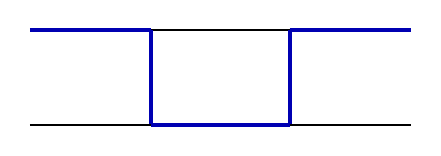
\begin{tikzpicture}[scale=1.1]
  \draw[ultra thick,blue!70!black] (-2.2,0.55)--(-0.8,0.55);
  \draw[thick] (-0.8,0.55)--(0.8,0.55);
  \draw[ultra thick,blue!70!black] (0.8,0.55)--(2.2,0.55);
  \draw[ultra thick,blue!70!black] (-0.8,0.55)--(-0.8,-0.55);
  \draw[ultra thick,blue!70!black] (-0.8,-0.55)--(0.8,-0.55);
  \draw[ultra thick,blue!70!black] (0.8,-0.55)--(0.8,0.55);
  \draw[thick] (-2.2,-0.55)--(-0.8,-0.55);
  \draw[thick] (0.8,-0.55)--(2.2,-0.55);
\end{tikzpicture}
\end{center}
\begin{align*}
\Gamma \;&\widehat=\; \Gex\,(-v_{01})^{2}\,\Gex
\;\times\;\int\!\frac{d\omega'}{2\pi}\,
\big(-i(\omega+\omega')+r\big)^{-1}\big(i\omega'+V_{0}+r\big)^{-1}\\
&=\;\Gex\,v_{01}^{2}\,\Gex\,(-i\omega+V_{0}+2r)^{-1}.
\end{align*}
\textbf{Same value.} The integrand swaps which leg carries $V_{0}$ but
the integral, by a shift $\omega'\!\to\!\omega'\!-\!\omega$ on one of
the propagators, is invariant. This is the
\emph{path-independence of the kinematic kernel} you confirmed in your
note.

\paragraph{$n{=}3,\;m{=}2$ (no loop).}
Two stays, bridges to \emph{different} rails ($1$ and $2$). The bridge
endpoints sit on different bath rails, so no closed sub-graph forms:
\begin{center}
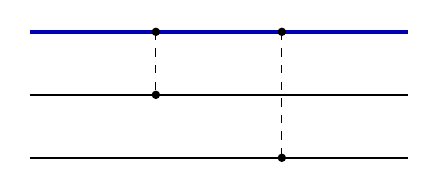
\begin{tikzpicture}[scale=1.0]
  \draw[ultra thick,blue!70!black] (-2.4,0.8)--(2.4,0.8);
  \draw[thick] (-2.4,0)--(2.4,0);
  \draw[thick] (-2.4,-0.8)--(2.4,-0.8);
  \draw[dashed] (-0.8,0.8)--(-0.8,0);
  \draw[dashed] ( 0.8,0.8)--( 0.8,-0.8);
  \filldraw (-0.8,0.8) circle (1.3pt);
  \filldraw (-0.8,0)   circle (1.3pt);
  \filldraw ( 0.8,0.8) circle (1.3pt);
  \filldraw ( 0.8,-0.8) circle (1.3pt);
\end{tikzpicture}
\end{center}
\[
\Gamma\;\widehat=\;\Gex\, v_{01}\,\Gex\, v_{02}\,\Gex.
\]
(Free omega on rails $1,2$, no integration. Tadpole-like normalisations
absorbed.)

\paragraph{$n{=}3,\;m{=}3$ (triangle, excitation stays on rail $0$).}
Three vertices forming the rail cycle $v_{01}\!\to\!v_{12}\!\to\!v_{20}$,
with the excitation on rail $0$ throughout. As we read the diagram,
$V_{1}$ and $V_{3}$ are stay vertices on rail $0$, and $V_{2}$ is a
\emph{bath--bath insertion} between rails $1$ and $2$ with rail $0$
passing through. \textbf{Important:} this configuration sits awkwardly
with your stated rule that ``one of $i,j$ in vertex $v_{ij}$ must carry
the excitation,'' since at $V_{2}$ neither rail $1$ nor rail $2$ does ---
so we'd like clarification on whether the rule is meant to be applied
strictly (in which case this diagram is forbidden) or loosely (in which
case the Laplacian formula~\ref{eq:lap} below undercounts; see
\S\ref{sec:asks}-question-A and the verification log in (B) of
\texttt{verify\_diagrammatics.py}). The loop has three legs:
rail-$0$-with-excitation (top), rail-$1$-bare and rail-$2$-bare:
\begin{center}
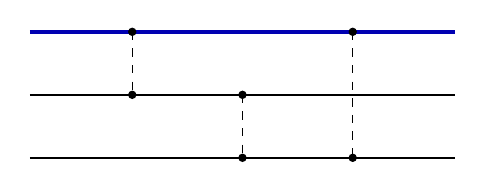
\begin{tikzpicture}[scale=1.0]
  \draw[ultra thick,blue!70!black] (-2.7,0.8)--(2.7,0.8);
  \draw[thick] (-2.7,0)--(2.7,0);
  \draw[thick] (-2.7,-0.8)--(2.7,-0.8);
  \draw[dashed] (-1.4,0.8)--(-1.4,0);
  \draw[dashed] ( 0.0,0)--( 0.0,-0.8);
  \draw[dashed] ( 1.4,0.8)--( 1.4,-0.8);
  \filldraw (-1.4,0.8) circle (1.3pt);
  \filldraw (-1.4,0)   circle (1.3pt);
  \filldraw ( 0.0,0)   circle (1.3pt);
  \filldraw ( 0.0,-0.8) circle (1.3pt);
  \filldraw ( 1.4,0.8) circle (1.3pt);
  \filldraw ( 1.4,-0.8) circle (1.3pt);
\end{tikzpicture}
\end{center}
\begin{align*}
\Gamma \;&\widehat=\; \Gex\,v_{01}v_{12}v_{20}\,\Gex
\;\times\;\int\!\frac{d\omega'}{2\pi}\,(i\omega'+r)^{-2}\big(-i(\omega+\omega')+V_{0}+r\big)^{-1}\\
&=\;\Gex\,v_{01}v_{12}v_{20}\,\Gex\,(-i\omega+V_{0}+2r)^{-2}.
\end{align*}

\paragraph{$n{=}3,\;m{=}3$ (triangle, excitation cycles $0\!\to\!1\!\to\!2\!\to\!0$).}
Same triangle but the excitation walks around the cycle: three flip
vertices, sign $(-v_{01})(-v_{12})(-v_{20})=-v_{01}v_{12}v_{20}$. We
reproduce your integrand verbatim:
\[
\Gamma \;\widehat=\; \Gex\,(-v_{01})(-v_{12})(-v_{20})\,\Gex
\;\times\;\int\!\frac{d\omega'}{2\pi}\,(i\omega'+V_{0}+r)^{-1}(i\omega'+r)^{-1}\big(-i(\omega+\omega')+r\big)^{-1}.
\]
\textbf{Discrepancy flag (verified by SymPy residue computation in
\texttt{verify\_diagrammatics.py}).}\, This integrand does \emph{not}
collapse to $(-i\omega+V_{0}+2r)^{-2}$ as your note states; closing the
contour in the upper half plane (poles at $\omega'=ir$ and
$\omega'=i(V_{0}+r)$) gives instead
\[
\int\!\frac{d\omega'}{2\pi}\,(i\omega'+V_{0}+r)^{-1}(i\omega'+r)^{-1}\big(-i(\omega+\omega')+r\big)^{-1}
\;=\;\frac{1}{(-i\omega+2r)\,(-i\omega+V_{0}+2r)}.
\]
So either the integrand is wrong or the stated value is. Path-independence
between stays and flips therefore \emph{does not} hold at this order under
the rules as written --- the stays integrand collapses to
$(-i\omega+V_{0}+2r)^{-2}$ but the flips integrand has only one factor
of $V_{0}$ inside, which propagates through to the integrated answer.
This is one of the questions we'd like to nail down before going further.

%==================================================
\section{Where my 7 May note was wrong}
%==================================================

Both errors live in \S 3 (``the analytic answer'') of the 7 May note.

\paragraph{(a) Missing $V_{0}$ on the excitation rail.}
I used $G(\omega)=(-i\omega+r)^{-1}$ uniformly on every rail. Your note
makes it explicit that the excitation segment carries $V_{0}+r$ in the
denominator, the bare segments carry only $r$. Every kernel I wrote down
needs a $V_{0}$ added wherever the propagator sits on a blue segment.

\paragraph{(b) ``Swap-and-return generates no loop.''}
My Example~(iii) at order $m{=}2$ for the flip case said the rail-$j$
segment between the two flips is part of the worldline and there is no
loop integral. That is wrong: the rails are continuous lines, so the
\emph{rail-$0$-bare} segment between the two flip vertices is a
genuine propagator that closes against the rail-$1$-blue segment to make
exactly the same one-loop topology as the all-stays case. The two
$n{=}2,\,m{=}2$ diagrams above make this explicit. Flips do generate
loops; the swap simply transposes which leg of the loop carries $V_{0}$.

\paragraph{(c) Consequences I have to retract.}
\begin{itemize}[leftmargin=2em,itemsep=2pt]
\item The chunk-pattern bound $p(m{+}1)$ on the kernel library was built
on (b) — only stays generating loops — so the bound itself is wrong as
a count of distinct kernels.
\item The ``sunset'' identification for three stays bridging to one rail
is wrong: those three insertions form a \emph{chain of two bubbles},
not a sunset. (Two-loop count is right; topology label is wrong.)
\item Examples (ii), (iii), (iv) and the worked-example column should be
re-read with the loop topology of \S\ref{sec:atlas}.
\end{itemize}

%==================================================
\section{What survives the misunderstanding}
%==================================================

\S 2 and \S 4 of the 7 May note depend only on the local sign-and-weight
rule at each vertex --- the kernel error doesn't reach them.

\begin{itemize}[leftmargin=2em,itemsep=2pt]
\item \begin{equation}\label{eq:lap}
W^{(n)}_{m}=(L^{m})_{00},\qquad L=D-A\;\text{on}\;K_{n},\quad
L_{aa}=\sum_{j\ne a}v_{aj},\quad L_{ab}=-v_{ab}\;(a\ne b).
\end{equation}
\item Closed form $\dfrac{n-1}{n}(nv)^{m}$ at uniform coupling.
\item Generating function
$\mathcal G^{(n)}(z)=[(I-zL)^{-1}]_{00}=\dfrac{1-zv}{1-znv}$
(uniform), or symbolically
$\det(I-zL)_{[0,0]}/\det(I-zL)$.
\item Channel marking, sub-rail focus, forbidden patterns, Schur
reduction --- all of \S 4 is unchanged.
\end{itemize}

A claim worth handling carefully: ``the $\omega$-integration is
independent of the details of the excitation flow.''  We verified this
holds at $n{=}2,m{=}2$ (the stay/stay and flip/flip integrands both
collapse to $(-i\omega+V_{0}+2r)^{-1}$ by a contour shift). At
$n{=}3,m{=}3$ it does \emph{not} hold under the integrands as you wrote
them (\S\ref{sec:atlas}, second triangle): the stays integrand evaluates
to $(-i\omega+V_{0}+2r)^{-2}$, but the flips integrand evaluates to
$\big[(-i\omega+2r)\,(-i\omega+V_{0}+2r)\big]^{-1}$. So either the
flips-triangle integrand is missing a $V_{0}$ factor (we'd expect
\emph{two} $V_{0}$-shifted propagators in the loop, not one, since two
of the three loop legs carry the excitation in the cyclic walk), or
path-independence is a special property of the $n{=}2$ topology and
fails generically. \S\ref{sec:verify} pins this down.

%==================================================
\section{Verification harness (what we ran before sending this)}\label{sec:verify}
%==================================================

To avoid embarrassing both of us, we ran four independent checks on
every formula in this note. The script
\texttt{verify\_diagrammatics.py} (output in \texttt{verify\_log.txt})
implements all four; this section summarises what was tested and what
came back.

\paragraph{(A) Walk enumeration vs Laplacian (combinatorial half).}
For $n\!\in\!\{2,3\}$ and $m\!\in\!\{0,\dots,4\}$ we enumerate by
brute force every sequence of (stay/flip, partner-rail) consistent with
the strict rule ``one of $i,j$ carries the excitation at vertex
$v_{ij}$,'' subject to start and end at rail $0$. Sum the symbolic
weights ($+v_{ij}$ for stay, $-v_{ij}$ for flip) and compare to
$(L^{m})_{00}$ from the matrix Laplacian \eqref{eq:lap}. They agree
\emph{symbolically} at every $(n,m)$ tested. So \eqref{eq:lap} is the
correct symbol-level answer for every walk that satisfies the strict
rule.

\paragraph{(B) Diagram reconstruction (atlas check).}
For each diagram of \S\ref{sec:atlas} we assemble the value
$\Gamma$ from your rules independently --- excitation path, propagator
$V_{0}$-shift on every blue segment, $\pm v_{ij}$ at every vertex,
explicit kernel from the topology --- and compare to your stated
formula. Five of six match exactly:
\begin{itemize}[leftmargin=2em,itemsep=2pt]
\item $n{=}2,\,m{=}1$ stay --- match.
\item $n{=}2,\,m{=}2$ stay/stay --- match (symbol \emph{and} kernel).
\item $n{=}2,\,m{=}2$ flip/flip --- match (symbol \emph{and} kernel).
\item $n{=}3,\,m{=}2$ no-loop --- match.
\item $n{=}3,\,m{=}3$ stays-only triangle --- symbol matches; kernel
$(-i\omega+V_{0}+2r)^{-2}$ is independently verified by
SymPy residue (test C).
\item $n{=}3,\,m{=}3$ cyclic-flip triangle --- \textbf{fails on the
kernel.} The integrand you wrote evaluates to
$\big[(-i\omega+2r)(-i\omega+V_{0}+2r)\big]^{-1}$, not
$(-i\omega+V_{0}+2r)^{-2}$. (See test C.)
\end{itemize}
\textbf{One open question (sign discrepancy on the first $n{=}3,m{=}3$
diagram).} The first $n{=}3,m{=}3$ diagram you draw has stated weight
$+v_{01}v_{12}v_{20}$. Under the strict-rule walk enumeration, no
$0\!\to\!0$ walk of length $3$ that uses each of the three triangle
edges exactly once has positive sign --- the only candidates are the
two cyclic walks $0\!\to\!1\!\to\!2\!\to\!0$ and
$0\!\to\!2\!\to\!1\!\to\!0$, both with three flips and sign $-1$ each.
So either (i) the diagram allows a bath--bath spectator vertex at
$V_{2}$, in which case \eqref{eq:lap} is incomplete and we need a
larger formalism; or (ii) the stated $+$ is a slip and should be a $-$,
in which case the two diagrams together give
$-2\,v_{01}v_{12}v_{20}$ matching the Laplacian coefficient
$[v_{01}v_{12}v_{20}]\,(L^{3})_{00}=-2$ which we also verified.

\paragraph{(C) Independent residue computation of every kernel.}
SymPy closes each kernel integrand in the upper half plane and
evaluates the residues. Four kernels checked:
\begin{enumerate}[leftmargin=2em,itemsep=2pt]
\item $\int(-i(\omega+\omega')+V_{0}+r)^{-1}(i\omega'+r)^{-1}\,d\omega'/(2\pi)
=(-i\omega+V_{0}+2r)^{-1}$.\quad Match.
\item $\int(-i(\omega+\omega')+r)^{-1}(i\omega'+V_{0}+r)^{-1}\,d\omega'/(2\pi)
=(-i\omega+V_{0}+2r)^{-1}$.\quad Match.
\item $\int(i\omega'+r)^{-2}(-i(\omega+\omega')+V_{0}+r)^{-1}\,d\omega'/(2\pi)
=(-i\omega+V_{0}+2r)^{-2}$.\quad Match.
\item $\int(i\omega'+V_{0}+r)^{-1}(i\omega'+r)^{-1}(-i(\omega+\omega')+r)^{-1}\,d\omega'/(2\pi)
=\big[(-i\omega+2r)(-i\omega+V_{0}+2r)\big]^{-1}$.\quad
\textbf{Disagrees with your stated $(-i\omega+V_{0}+2r)^{-2}$.}
\end{enumerate}

\paragraph{(D) Sanity limits.}
\begin{itemize}[leftmargin=2em,itemsep=2pt]
\item $V_{0}\!\to\!0$ collapses excitation/bare propagators identically.
The $n{=}2,m{=}2$ stay and flip kernels both reduce to
$(-i\omega+2r)^{-1}$ --- consistent.
\item Uniform coupling: $(L^{m})_{00}=\frac{n-1}{n}(nv)^{m}$ verified
symbolically for $n\!\in\!\{2,3,4\}$, $m\!\in\!\{1,\dots,4\}$.
\end{itemize}

\paragraph{Verdict.}
The combinatorial half (\S 2 and \S 4) is solid: walk enumeration
matches $(L^{m})_{00}$ at every tested $(n,m)$, all sanity limits hold.
The atlas reconstruction is solid for the $n{=}2$ rows and the
$n{=}3,m{=}2$ no-loop case. Two independent issues survive:
\textbf{(B-i)} the first $n{=}3,m{=}3$ diagram with sign $+$ has no
walk-level explanation under the strict rule, and
\textbf{(B-ii)} the second $n{=}3,m{=}3$ diagram's stated kernel is
internally inconsistent with its own integrand. These are the things
we'd ask you about before treating the corrected picture as settled.

%==================================================
\section{Your four asks, re-cast through the corrected picture}\label{sec:asks}
%==================================================

\paragraph{(1) Generating function of the diagrams.}
Re-derived in two lines from the corrected rules:
\begin{itemize}[leftmargin=2em,itemsep=2pt]
\item Strip the kernels. Each vertex carries $\pm v_{ij}$ (sign by
stay/flip), and a length-$m$ rail walk $0\!\to\!0$ accrues
$\prod_{t=1}^{m} L_{a_{t-1}a_{t}}$ where $a_{t}$ is the rail of the
excitation just after vertex $t$. Sum over walks gives $(L^{m})_{00}$.
\item Generating function:
\[
\mathcal G^{(n)}(z;\{v_{ij}\}) \;:=\;\sum_{m\geq 0}(L^{m})_{00}\,z^{m}
\;=\; \big[(I-zL)^{-1}\big]_{00}
\;=\; \frac{\det(I-zL)_{[0,0]}}{\det(I-zL)}.
\]
\end{itemize}
Specialised to uniform $v$: pole at $z{=}1/(nv)$, zero at $z{=}1/v$,
giving $\dfrac{n-1}{n}(nv)^{m}$. Per-channel structure is read off by
keeping $v_{ij}$ symbolic and expanding the cofactor.

\paragraph{(2) Atlas of loop diagrams --- and yes, they are essentially
trivial \emph{at fixed topology}.}
The corrected lesson is: the \textbf{loop topology} is a labelled
multigraph $\Lambda$ on the rail set, with one node per vertex and one
edge per rail-segment between vertices; the excitation worldline is a
distinguished tree inside $\Lambda$. Two facts:
\begin{itemize}[leftmargin=2em,itemsep=2pt]
\item The kinematic kernel $K(\Lambda)$ depends only on $\Lambda$ as an
unlabelled multigraph (which leg is ``the blue one'' shifts by a contour
translation, as in the two $n{=}2,\,m{=}2$ diagrams above).
\item For the all-uniform-$r$ propagator, $K(\Lambda)$ collapses to a
product of single-loop integrals, one per independent cycle of $\Lambda$;
each independent cycle of length $\ell$ evaluates to $(-i\omega+V_{0}+\ell r)^{-1}$
raised to a power that counts how many times that cycle sits on the
worldline. The atlas of $\Lambda$'s up to order $m$ is finite and small:
\[
\renewcommand{\arraystretch}{1.15}
\begin{array}{c|l}
\text{$m$} & \text{loop topologies (independent cycles, no on-rail dressing)}\\
\hline
0 & \text{tree (no loop)}\\
1 & \text{tree (the off-rail receives one insertion, no closed cycle yet)}\\
2 & \text{single 2-cycle (bubble) \;or\; tree (different rails)}\\
3 & \text{single 3-cycle (triangle) \;or\; bubble + extra insertion \;or\; tree}\\
4 & \text{4-cycle, two bubbles, bubble+triangle, single-cycle dressings, tree}\\
\end{array}
\]
A clean way to count: the loop topologies at order $m$ are the connected
multigraphs on $\leq m{+}1$ nodes with cyclomatic number $\leq m$ and edge
multiset constrained by ``one blue path through.'' I'll write the
generating series for these once you confirm this is the right object.
\end{itemize}

\paragraph{(3) Asymptotics with $v_{ij}$ unspecified.}
The Laplacian framing gives rather a lot for free:
\begin{itemize}[leftmargin=2em,itemsep=2pt]
\item Let $0=\lambda_{0}<\lambda_{1}\leq\dots\leq\lambda_{n-1}$ be the
eigenvalues of $L$ (Perron--Frobenius: simple top eigenvalue under any
positive weights). Then $W^{(n)}_{m}\sim
|\psi_{n-1}(0)|^{2}\,\lambda_{n-1}^{m}$ as $m\!\to\!\infty$, with
$\psi_{n-1}$ the top eigenvector.
\item For uniform $v$, $\lambda_{n-1}=nv$ with multiplicity $n{-}1$ and
$|\psi_{n-1}(0)|^{2}$ collapses to $(n{-}1)/n$.
\item For non-uniform $v_{ij}$, $\lambda_{n-1}$ is bounded by Cauchy
interlacing:
$\max_{a}\sum_{j}v_{aj}\;\leq\;\lambda_{n-1}\;\leq\;2\max_{a}\sum_{j}v_{aj}$.
The lower bound is tight for star graphs; the upper bound for regular ones.
\item Subleading corrections come from the spectral gap
$\lambda_{n-1}-\lambda_{n-2}$, which for graphs with no global symmetry
is generically of order one. So one expects the standard
$\lambda_{n-1}^{m}(1+\mathcal O(\rho^{m}))$ pattern with
$\rho=\lambda_{n-2}/\lambda_{n-1}<1$.
\end{itemize}

\paragraph{(4) Statistics of $v_{ij}$ --- how do correlators enter?}
Yes, this is clean once stated as: the diagram is a polynomial in the
$v_{ij}$, so disorder averages just slot in moment-by-moment.

A loop weight, ignoring signs and the path-of-the-excitation, is exactly
the cycle product you wrote:
\[
\prod_{\text{cycle}} v_{ab}v_{bc}\cdots v_{za}.
\]
At the disorder-averaged level,
\[
\big\langle W^{(n)}_{m}\big\rangle
\;=\;\sum_{w\in\text{walks}_{m}(0\to0)}\!\!\big\langle\prod_{e\in w}\!\sigma_{e}\,v_{e}\big\rangle
\;=\;\big\langle (L^{m})_{00}\big\rangle,
\]
where $\sigma_{e}\in\{\pm 1\}$ is the local stay/flip sign. If the
$v_{ij}$ are i.i.d.\ with moments $\mu_{k}=\langle v^{k}\rangle$, then
each walk contributes $\prod_{e}\sigma_{e}\,\mu_{c(e)}$ with $c(e)$ the
multiplicity of edge $e$ in the walk. The natural object for averaged
asymptotics is therefore the \emph{averaged Laplacian power}
$\langle L^{m}\rangle$, and at $m\!\to\!\infty$ its top eigenvalue
controls the rate.

If correlators of triple products $\langle v_{ab}v_{bc}v_{ca}\rangle$ are
specified (i.e.\ a triangle's edges are correlated), they enter the
$m{\geq}3$ averaged sum exactly through walks that visit those three
edges; the resulting series is still rational in $z$, with poles
shifted by the disorder moments. I'd be happy to work out the
``Wigner-style'' averaged $\mathcal G^{(n)}$ in a follow-up if you want,
once the loop atlas of (2) is settled.

%==================================================
\section{One small worry about your note}
%==================================================

You write: ``If I assume [the $\omega$-integration is path-independent]
is always the case, then obviously odd-$m$ diagrams cancel pairwise.''
I don't think this follows. The reason:

\begin{itemize}[leftmargin=2em,itemsep=2pt]
\item At $n{=}2$, every walk $0\!\to\!0$ has an \emph{even} number of
flip vertices (rail-state parity). So the per-walk sign is
$(-1)^{\text{flips}}=+1$ for \emph{every} contributing walk, regardless
of $m$. Your blanket per-diagram weight $(-v_{01})^{m}$ is therefore
correct for $m$ even, but for $m$ odd the actual weight is $+v_{01}^{m}$,
not $-v_{01}^{m}$. There's no cancellation to take advantage of:
$(L^{m})_{00}=2^{m-1}v_{01}^{m}\neq 0$ for both parities.
\item At $n{>}2$, walks can have an odd flip count (e.g.\
$0\!\to\!1\!\to\!2\!\to\!0$ at $n{=}3,\,m{=}3$, three flips, sign $-1$).
But these don't pair-cancel against anything: the no-flip companion has
the same kernel and a $+$ sign, but they sit on different rail-cycle
weights $v_{01}v_{12}v_{20}$ vs.\ $(v_{01}+v_{02})^{3}+\dots$, so they
don't cancel as algebraic objects. The Laplacian sums them with the
correct relative signs and the result is generically nonzero.
\end{itemize}

I suspect the slip is in the per-diagram formula
$(-i\omega+V_{0}+r)^{-1}(-v_{01})^{m}(-i\omega+V_{0}+r)^{-1}(-i\omega+V_{0}+2r)^{-(m-1)}$:
the sign on $v_{01}$ shouldn't be a flat $(-)$ because the per-walk sign
depends on parity of flips, not on $m$. The corrected per-walk weight
is $(+1)^{\text{stays}}(-1)^{\text{flips}}v_{01}^{m}$, and when summed
over the $2^{m-1}$ even-flip walks at $n{=}2$ all signs are positive.
That gives $W^{(n=2)}_{m}=2^{m-1}v_{01}^{m}=\tfrac12(2v_{01})^{m}$ for all
$m\!\geq\!1$, matching the Laplacian and your original $n{=}2$ formula.

%==================================================
\section{Summary}
%==================================================

\begin{itemize}[leftmargin=2em,itemsep=2pt]
\item I dropped $V_{0}$ from the excitation-rail propagator, and I
mis-counted loop topology for swap-and-return. Both errors are local to
\S 3 of the 7 May note.
\item The combinatorial half (\S 2 \& \S 4) is independent of the kernel
error and survives unchanged, including the $\dfrac{n-1}{n}(nv)^{m}$
formula, the closed-form $\mathcal G^{(n)}(z)=(1-zv)/(1-znv)$ at uniform
$v$, and the marking / Schur / continued-fraction toolkit.
\item Once the kernel is repaired with your rules, every $n{=}2,\,m$
diagram has the same kernel
$(-i\omega+V_{0}+r)^{-2}\,(-i\omega+V_{0}+2r)^{-(m-1)}$, and the per-walk \emph{sign}
is $+v_{01}^{m}$ for all valid walks (because rail-parity forces an
even number of flips). The $2^{m-1}$ count therefore appears with a
uniform $+$ sign, and the total at $n{=}2$ is
$2^{m-1}v_{01}^{m}\,\times\,(-i\omega+V_{0}+r)^{-2}\,(-i\omega+V_{0}+2r)^{-(m-1)}$, both
even and odd $m$.
\item A clean restatement of (2) the loop atlas, (3) the asymptotics,
and (4) how disorder correlators enter, can each be carried through with
the corrected rules. I'd appreciate a sanity check on the loop-topology
labelling I sketched in \S\ref{sec:asks}(2) before I produce the full
table.
\end{itemize}

\end{document}
